\section{Markov Chains \skript{103-148}}
\textbf{The future is independent of the past, given the present}:\\
In other words, the present state is enough to determine the statistics of the future.
\begin{equation}
	P\left(X(t_n)\leq x_n|\{X(t)\}_{t\leq t_{n-1}}\right)=P\left(X(t_n)\leq x_n|X(t_{n-1})\right)\nonumber
\end{equation}

\subsection{Discrete-time Markov chains \skript{103-121}}
\begin{equation}
	P\left(X_{n+1}=x_{n+1}|X_n=x_n,\ldots,X_0=x_0\right)=P\left(X_{n+1}=x_{n+1}|X_n=x_n\right)\nonumber
\end{equation}

 If the transition probabilities do not depend on time $k$ we say that $X$ is a \textbf{time-homogeneous Markov chain} and we use the notation.

\begin{equation}
	p_{ij}=P(X_{k+1}=j|X_k=i) \qquad \text{(state i $\rightarrow$ state j)}\nonumber
\end{equation}

The associated matrix, indexed by state space $S=\{1,2,\ldots,n\}$ is the \textbf{transition matrix}:
\begin{equation}
	P=\begin{pmatrix}
		p_{11} &\cdots & p_{1n}\\
		\vdots& & 	\vdots\\
		p_{n1} &\cdots & p_{nn}\\
	\end{pmatrix}\nonumber
\end{equation}

An other way to specify the transition probabilities is with a \textbf{state transition diagram}:

\begin{minipage}{0.4\textwidth}
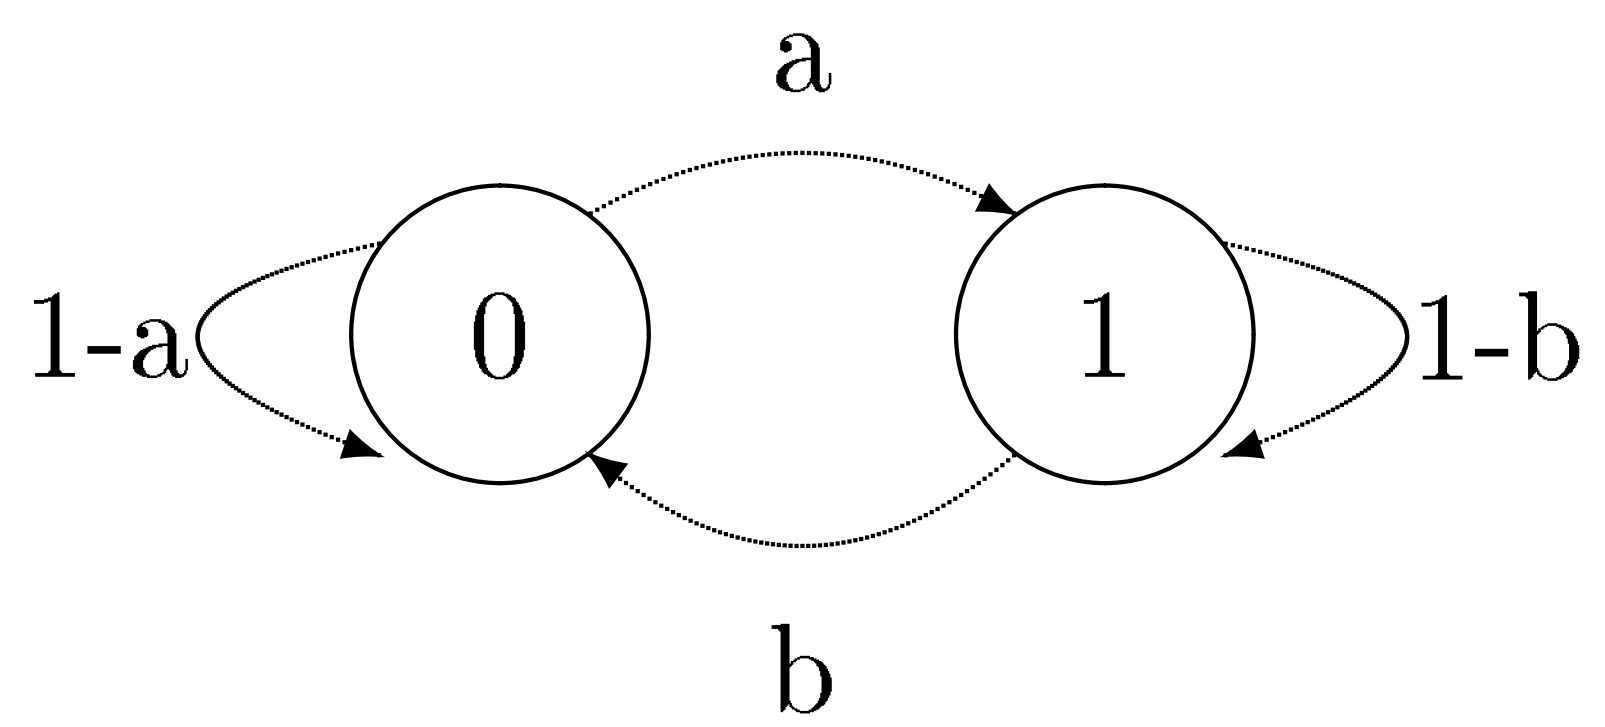
\includegraphics[width=0.8\linewidth]{./Content/Markov/statediag}
\end{minipage}
\begin{minipage}{0.4\textwidth}
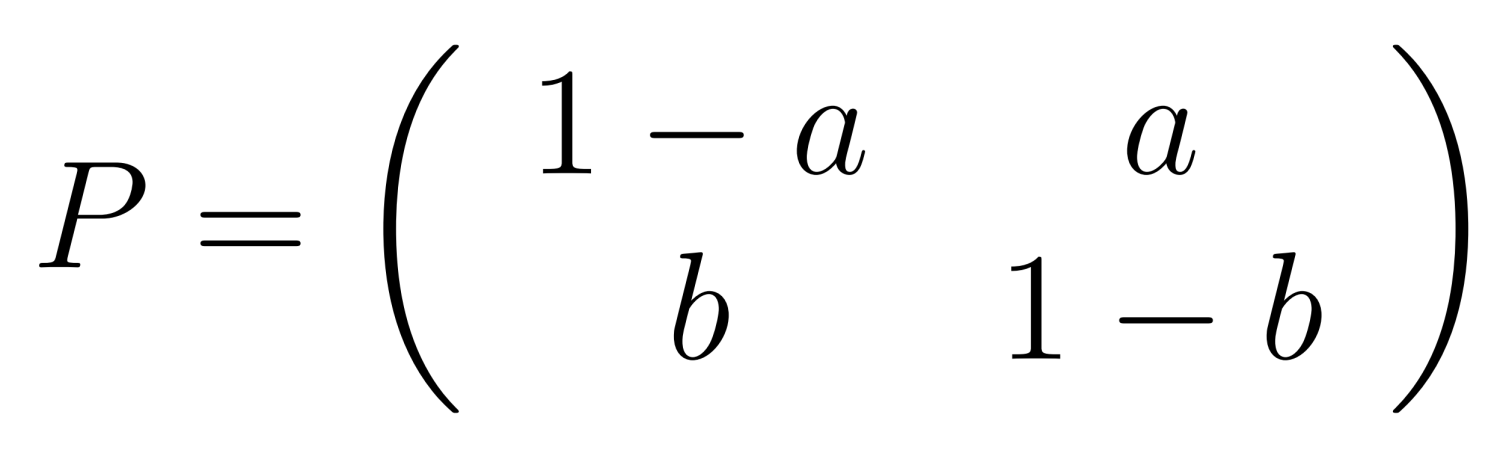
\includegraphics[width=0.8\linewidth]{./Content/Markov/statetab}
\end{minipage}
\hfill


\subsubsection{The Chapmann-Kolmogorov equations \skript{107-108}}
The (exactly) $m$ step transition probabilities of a homogeneous Markov chain $X$ are definde by: 

\begin{equation}
	p_{ij}^{(m)}=P(X_m=j|X_0=i)	\\ 
	p_{ij}^{(n+m)}=\sum\limits_k{p_{ik}^{(n)}p_{kj}^{(m)}}\\
	P^{n+m}=P^nP^m\nonumber
\end{equation}


\subsubsection{The stationary distribution \skript{109}}

The probability distribution of a Chain with initial probability $\nu$ is:
\begin{equation}
	\boxed{p_{j}^{(n)}=\sum\limits_i{\nu_i p_{ij}^{(n)}}} \quad
	\boxed{p^{(n)}=\nu P^{n}}
\end{equation}

The stationary distribution ($n\rightarrow \infty$) of a Chain is:
\begin{equation}
	\boxed{\pi_{j}=\underbrace{\sum\limits_k{\pi_k p_{kj}}}_{\text{probabilities to enter state }j},~~ \pi_j\geq 0 ~~ and ~~ \sum\limits_k{\pi_j}=1}\nonumber \quad
	\boxed{\pi=\pi P}
\end{equation}

$\pi$ is a eigenvector of $P$ with eigenvalue $1$\\

The equations below are to solve to get the eigenvector $\pi$:

\begin{equation}
\bm{\pi}=\bm{\pi}\cdot \bm{P}=\begin{pmatrix}\pi_1& \ldots & \pi_n\end{pmatrix}=\begin{pmatrix}\pi_1& \ldots & \pi_n\end{pmatrix}\cdot\begin{pmatrix}
		p_{11} &\cdots & p_{1n}\\
		\vdots& & 	\vdots\\
		p_{n1} &\cdots & p_{nn}\\
	\end{pmatrix}\qquad and\qquad\pi_1+\ldots+\pi_n=1\nonumber
\end{equation}

\begin{itemize}
\item $\pi_i$ is the time (in \%) spent in state $i$
\end{itemize}

TI-89 can solve matrix equations only with Simult.Eqn.Solver. $\bm \pi$ can be found by calculating 
$\bm P^{100} \approx \bm P^\infty = \begin{bmatrix}\pi_1 & \ldots & \pi_n\\ \vdots &\ddots &\vdots\\\end{bmatrix}$

\subsubsection{Some Definitions \skript{112}}
\begin{itemize}
\item We say a state $j\in S$ is \textbf{accessible} from a fixed state $i\in S$ if there exists $n\geq 0 $ such that $p_{ij}^n>0$. We write $i\rightarrow j$
\item If $j$ is acessible from $i$ and $i$ from $j$, we say that $i$ and $j$ \textbf{communicate} and write $i \leftrightarrow j$
\item $X$ is \textbf{irreducible} if all states communicate with each other. Note that this is equivalent with the existene of a path in the state transition diagram from $i$ to $j$ and back from $j$ to $i$ for all pairs of state $i$, $j$.\\
Example: $0 \to 1 \to 2 \to 3 \to 0$

An irreducible Markov chain has \textbf{only one stationary distribution}.
(Wenn man einen Weg vom ersten Zustand, durch alle anderen Zustände und wieder zurück zum ersten Zustand mit einer Wahrscheinlichkeit ungleich Null findet.)
\end{itemize}

Given a Markov Chain $X$ with state space $S$. For any state we let $f_i$ be the probability of returning to the state $i$ if the chain starts at $i$.

\begin{itemize}
\item We say that a state $i \in S$ is \textbf{recurrent} if $f_i=1$. Hence, with probability $1$ the process will eventually reenter the state $i$. At least one state have to be recurrent. $f_i=P($return to i$|$in i$)$
\item We say that a state $i \in S$ is transient if $f_i<1$. Hence, with strictly positive probability $1-f_i$ the process will never again reenter the state $i$.
\item If state $i$ is recurrent (resp. transient) then all states communicating with $i$ are also recurrent (resp. transient).
\end{itemize}


If the transition matrix P of a Markov chain is such that exists $m \in \mathbb{N}$ with the property that all entries of $P^m$ are strictly positive then:
\begin{itemize}
\item There exists one unique stationary distribution $\pi$
\item For every initial condition $\lim\limits_{n\rightarrow \infty}{\nu(n)}=\lim\limits_{n\rightarrow \infty}{\nu(0)P^n}=\pi$
\item The rows of $P^n$ converge towards the stationary vector $\pi$
\end{itemize}

\vfill

\subsubsection{Random walks on graphs}

\textbf{Definition: } A graph $G$ consists of a vertex set $V$ and a edge set $E$ where each edge is an unordered pair of vertices.

\vspace{0.25cm}

\begin{minipage}{0.15\textwidth}
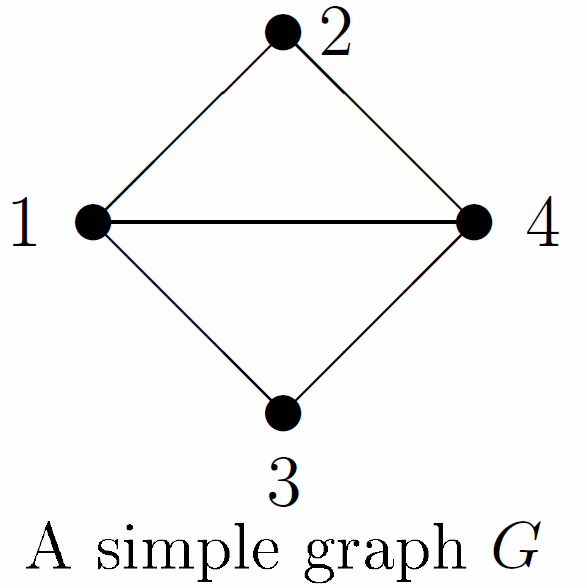
\includegraphics[width=\textwidth,trim= 0cm 2cm 0cm 0cm,clip]{./Content/Markov/simpleGraph}
\end{minipage}
\hfill
\begin{minipage}{0.8\textwidth}
This picture shows a simple-graph $G=(V,E)$ with Vertex set $V=\{1,2,3,4\}$ and edge set $E=\{\{1,2\},\{1,3\},\{1,4\},\{2,4\},\{3,4\}\}$. (Simple graph because no loops and no multiple edges). The multi-graph with loops and multiple edges don't considered here.
\end{minipage}

%\vspace{0.25cm}

\begin{itemize}
	\item \textbf{The degree} $d_i$ of a vertex $i \in V$ is the number of edges incident to the vertex $i$. In the example above it is $d_1=d_4=3$ and $d_2=d_3=2$.
	\item \textbf{The volume} of a subset of vertices $S \subset V$ is \qquad $\text{Vol}(S)=\sum\limits_{i\in S}^{} d_i$
	\item \textbf{A path} from $i$ to $j$ of length $n$ in $G$ is an ordered sequence of distinct vertices $i=v_0,v_1,\ldots,v_n=j$ satisfying $\{v_k,v_{k+1}\} \in E$ for $k=0,1,\ldots,n-1$.
	\item A graph is \textbf{connected} if for any two vertices $i$ and $j$, there is a path from $i$ to $j$.
	\item The \textbf{adjacency matrix} $\bm{A}=(a_{ij})$ pf a simple graph $G$ on $n$ vertices is the $n \times n$  matrix is: $\mtwopartdef{1}{\{i,j\} \in E}{0}$
	\item The \textbf{degree matrix} $\bm{D}$ of a simple graph G on n vertices is the $n \times n$ diagonal matrix $\bm{D}=diag(d_1,\ldots,d_n)$ where $d_i$ is the degree of vertex $i$
	\item The \textbf{transition probabilities} of the random walk on graph G is: $\bm{P}=\bm{D^{-1}A}$ \qquad $p_{ij}=(\bm{P})_{ij}=\mtwopartdef{1/d_i}{\{i,j\} \in E}{0}$
	\item \textbf{Example} for graph G:\\
	\begin{equation}
		\bm{A}=\begin{pmatrix}
			0 & 1 & 1 & 1\\
			1 & 0 & 0 & 1\\
			1 & 0 & 0 & 1\\
			1 & 1 & 1 & 0
		\end{pmatrix}\\
		\bm{D}=\begin{pmatrix}
			3 & 0 & 0 & 0\\
			0 & 2 & 0 & 0\\
			0 & 0 & 2 & 0\\
			0 & 0 & 0 & 3
		\end{pmatrix}\\
		\bm{P}=\begin{pmatrix}
			0 & 1/3 & 1/3 & 1/3\\
			1/2 & 0 & 0 & 1/2\\
			1/2 & 0 & 0 & 1/2\\
			1/3 & 1/3 & 1/3 & 0
		\end{pmatrix}\\
	\end{equation}\nonumber
\end{itemize}

\textbf{Theorem: } Under ergodic conditions we have for \textbf{any initial condition} $\nu: V \rightarrow \mathbb{R}, \sum\limits_{i}^{}{\nu_i=i}$ that the distribution after $k$ steps, $\nu\bm{P}^k$, converges to the unique distribution $\pi$:

\begin{equation}
	\boxed{\lim\limits_{k \rightarrow \infty}{\big(\nu\bm{P}^k\big)_i}=\pi_i=\frac{d_i}{\sum\limits_{j}^{}{d_j}}}\\
	\text{convergence speed:\qquad} ||\nu\bm{P}^2-\pi || \leq \e^{-s\lambda^{'}}\frac{\underset{i}{max}\sqrt{d_i}}{\underset{j}{min}\sqrt{d_j}}\nonumber\\
\end{equation}

with $\lambda^{'}=min\{\lambda_2,2-\lambda_n\}$ where $\lambda_2$ is the second largest and $\lambda_n$ the smallest eigenvalue of $\bm{P}$.\\

\textbf{For the above example of simple-graph $G$: } 

\renewcommand{\arraystretch}{2.0}
\begin{tabular}{ll}
\textbf{Stationary distribution: }& $\pi_1=\frac{d_1}{\sum\limits_j{d_j}}=\frac{3}{3+2+2+3}=\frac 3 {10} \qquad \pi_2=\frac{d_2}{\sum\limits_j{d_j}}=\frac{2}{3+2+2+3}=\frac 2 {10}  \qquad \pi_3=\frac 2 {10}  \qquad \pi_4=\frac 3 {10}$\\
Eigenvalue: & $|\bm{P}-\lambda\bm{I}|=0\quad \rightarrow \quad \lambda_i\qquad \text{for the example: }\lambda_1=1\quad\lambda_2=0\quad\lambda_3=-1/3\quad\lambda_4=-2/3$\\
Exponent e-function: & $\lambda^{'}=min\{\lambda_2,2-\lambda_n\}=min\{0,2-(-2/3)\}=0$\\
\textbf{Convergence speed: }& $||\nu\bm{P}^2-\pi || \leq \e^{-s\lambda^{'}}\frac{\underset{i}{max}\sqrt{d_i}}{\underset{j}{min}\sqrt{d_j}}=\e^{-s\cdot 0} \frac{\sqrt{3}}{\sqrt{2}}=\frac{\sqrt{3}}{\sqrt{2}}$
\end{tabular}
\renewcommand{\arraystretch}{1.0}












